\documentclass{article}

%Packages
\usepackage{graphicx}
\usepackage{grffile}
\usepackage{float}

%Margins
\usepackage[
	margin=2cm,
	includefoot
	]{geometry}

%Images
\usepackage{graphicx}

\graphicspath{{images/}}

%Headers and Footers
\usepackage{fancyhdr}
\pagestyle{fancy}
\fancyhead{}
\fancyfoot{}
\fancyfoot[R]{\thepage}
\renewcommand{\headrulewidth}{0pt}
\renewcommand{\footrulewidth}{0pt}


%Details
\title{
Software Requirements Specification and 
Technology Neutral Process Design
(University of Pretoria - Postgraduate Paper Interaction Portal)
}
\date{2016-02-15}
\author{Team Juliet}

%Document start
\begin{document}

%Title Page
\begin{titlepage}
	\begin{center}
		
\includegraphics[width=10cm]{UP.jpg}  \\
		[1cm]
		\line(1,0){300} \\
		[0.4cm]
		\textsc{\huge
			Software Requirements Specification and 
			Technology Neutral Process Design
			(University of Pretoria - Postgraduate Paper Interaction Portal)
		} \\
		[0.1cm]
		\line(1,0){300} \\
		[0.4cm]
		\textsc{\Large
			Team Juliet
		} \\

	\end{center}
	\begin{flushright}
	\textsc{\Large
	Quinton Weenink\\ 
	u13176545\\
	Vuyani Shabangu\\
	u11171139\\
	Ruan Klinkert\\
	u14022282\\
	Reinhardt Cromhout\\
	u14009936\\
	Rohan Chhipa\\
	u14188377\\
	Brandon Wardley\\
	u29005150\\
	}
	\end{flushright}
\end{titlepage}

%Table of contents
\tableofcontents
\thispagestyle{empty}
\cleardoublepage

%Content
\setcounter{page}{1}
\section{Introduction}
%\lable{sec:intro} for some readon i cant get the lables to work maybe you guys will have some luck
The purpose of this document is to describe the requirements of the “Postgraduate Paper Interaction Portal” application, by illustrating the purpose and uses of the system, as well as the development of the system. The system constraints, interface and various interactions will also be discussed, and testable quality requirements will be provided where applicable.

\section{Vision}
%\lable{sec:vision}
The “Postgraduate Paper Interaction Portal” is an application which allows the effective management of research groups, research projects, and researchers themselves, using either a web interface, or an android application. The application will allow the storage of metadata pertaining to papers which are being written or have been written, the authors who are involved with these papers, as well as the various publications to which these papers will be submitted. The application is intended for internal use by the University of Pretoria’s Department of Computer Science, and should be as simple and lightweight as possible.\\


A system administrator will be in charge of managing the system, and as such they can add and remove users, as well as change metadata when and where necessary. The administrator will also ensure that the system is properly audited, with all changes being recorded by the system itself.\\


The Head of Department (HoD) can view the status of all papers within the department, as well as their metadata, such that the progress and status of these papers can be tracked. The HoD can also view the statistics of each department, showing the number of researchers within that department, the number of publishing units that department has accrued, the number of papers they have released, and what the various performance goals of that department are.\\


%****(separate the responsibility of removing users to the admin only?)****

Research leaders are in charge of all the researchers within their specific research group. They can view the status and progress of all papers to be published under their group, as well as the metadata associated with each paper. Research leaders can view the details of each researcher within their group, as well as add new researchers to their group as needed.\\


A normal user within the system is a researcher who falls under the authority of a specific research leader. The user can view the metadata of each paper of which they are an author or co-author, and are also able to change these details as necessary by editing stored data, changing the progress report of the paper, or changing the status of the paper. The user can also create new papers, provided that they are either an author or co-author of said paper.\\


Each user within the system is responsible for entering the required metadata for each user, researcher, paper or publication goal they introduce into the system. The system will store each new entry, such that it might quickly be retrieved for future use, thus saving the users time when entering data. Papers may not be deleted from the system, and each entry or change within the system must be recorded.\\


\newpage
\section{Background}
%\lable{sec:background}
The need for the “Postgraduate Paper Interaction Portal” became apparent after it was found that the system currently in use by the University of Pretoria’s Department of Computer Science was no longer sufficient to effectively cater to the needs of the department. In its current state, this system consisted out of a single spreadsheet into which all the various details pertaining to research groups, projects, researchers and publications were inserted. These details were stored in a number of tables, and, using various mathematical formulae, a number of useful statistics were shown, usually pertaining to the number of publication units earned by researchers versus their goal. Whilst this system has the benefit of making all the stored information available at a single glance, the way in which this information is displayed is cluttered and confusing, a problem which becomes more apparent as the amount of stored information increases.\\


Research and the publication of findings is a crucial part of the department’s work, and as such, a request was made for the development of an application which would allow the researchers and staff within the department to easily track and manage the details of their research projects. This functionality extends to the ability to easily add new projects, researchers and publishing goals into the system, with much of the management and processing of this information now being handled by the application itself, as opposed to the users.\\


If it is found that this system succeeds as an improvement over the old system, and that research personnel find that it provides a quality of life improvement when managing research projects, the application may be further improved and distributed such that it may be used by other departments within the University of Pretoria. Once it has been established that the application can be used by multiple departments, and that it notably simplifies and improves the research management process, the application may be marketed for use in other institutions.




\section{Functional requirements and application design}
%\lable{sec:funcreq}
In order to represent all of the use cases associated with the system we have divided the system up into sections that will indicate all of the use cases associated with each and how they include or expand upon other use cases.
	

\subsection{Operator subsystem}
	\subsubsection{Use cases}

		\begin{flushleft}
			\textbf{Critical}
				\begin{itemize}
	  				\item Add drone
	  				\item Remove drone
					\item Assign research group leader
					\item View research group unit score
				\end{itemize}

			\textbf{Nice-To-Have}
				\begin{itemize}
	  				\item Edit drone
				\end{itemize}
		\end{flushleft}

	\subsubsection{Services Contracts}

		\begin{figure}[H]
			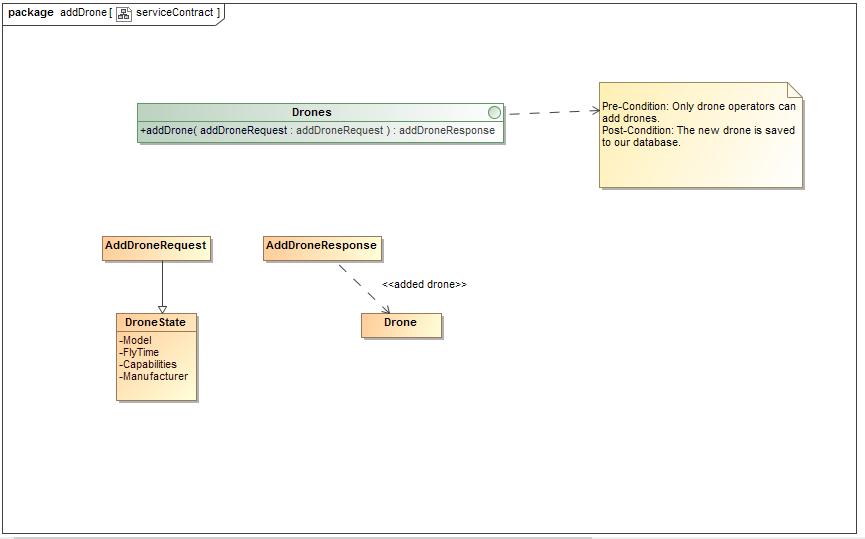
\includegraphics[width=\textwidth]{SC_add.png}  \\
			\caption{Services Contract : addDrone}
		\end{figure}
		\begin{figure}[H]
			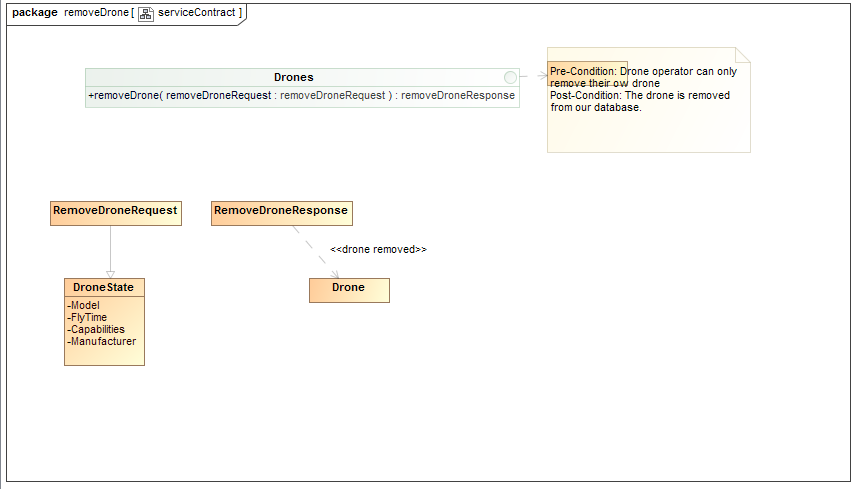
\includegraphics[width=\textwidth]{sc_delete.png}  \\
			\caption{Services Contract : removeDrone}
		\end{figure}
		\begin{figure}[H]
			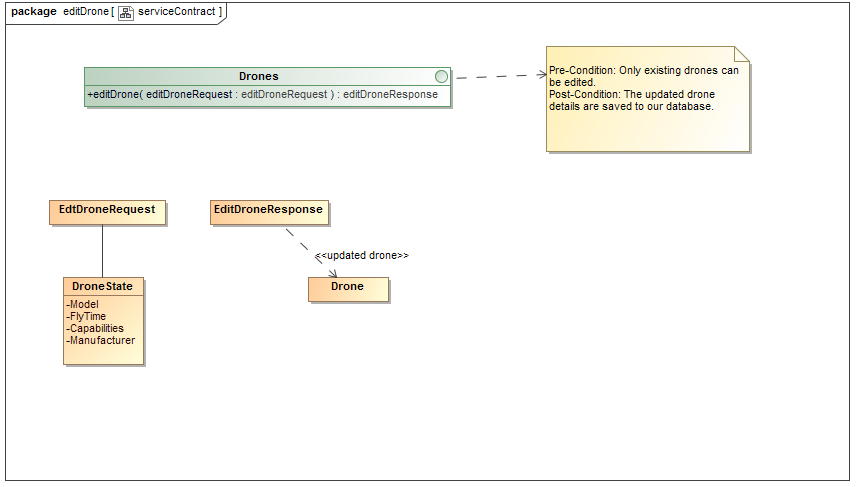
\includegraphics[width=\textwidth]{sc_edit.png}  \\
			\caption{Services Contract : editDrone}
		\end{figure}

	\subsubsection{Required functionality}
	
		\begin{figure}[H]
			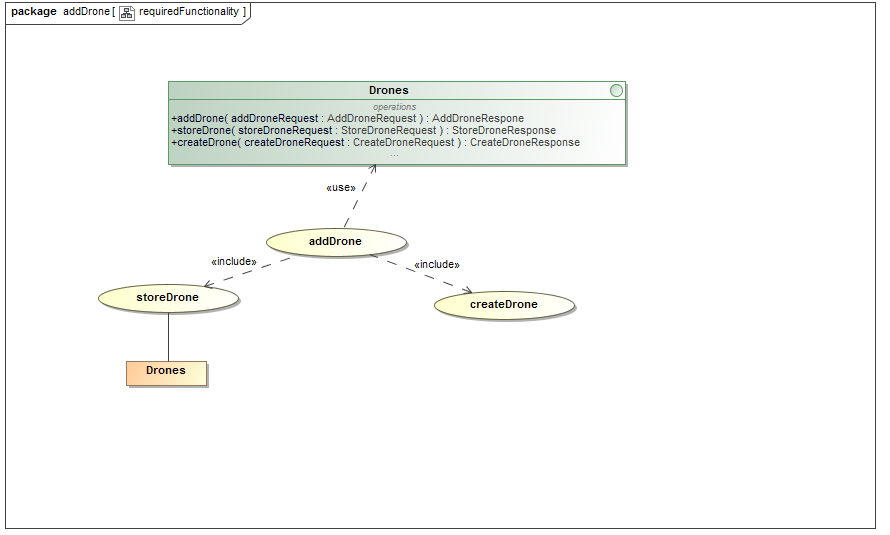
\includegraphics[width=\textwidth]{rf_add.png}  \\
			\caption{Functional Requirements : addDrone}
		\end{figure}
		\begin{figure}[H]
			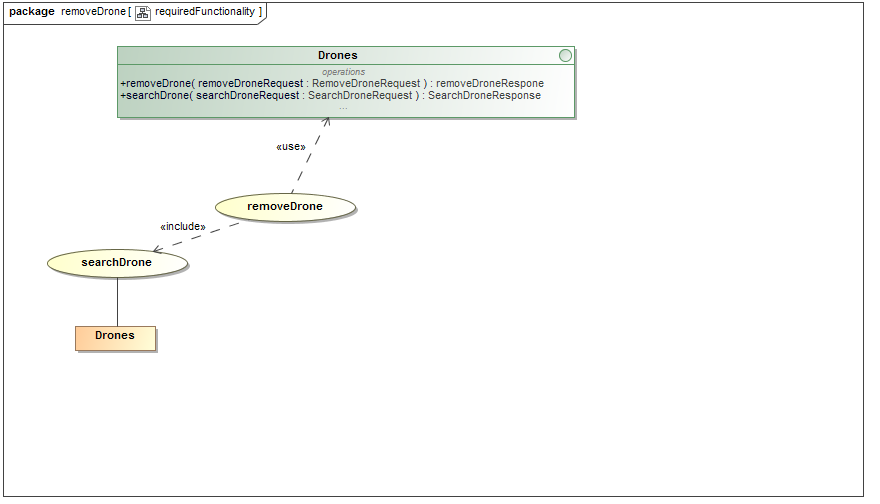
\includegraphics[width=\textwidth]{rf_remove.png}  \\
			\caption{Functional Requirements : removeDrone}
		\end{figure}
		\begin{figure}[H]
			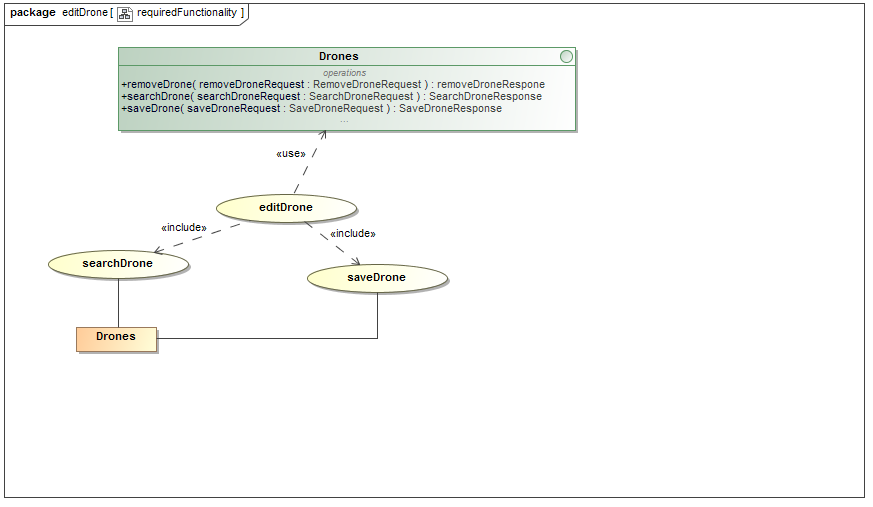
\includegraphics[width=\textwidth]{rf.png}  \\
			\caption{Functional Requirements : editDrone}
		\end{figure}
	

	\subsubsection{Process specifications}
	
		\begin{figure}[H]
			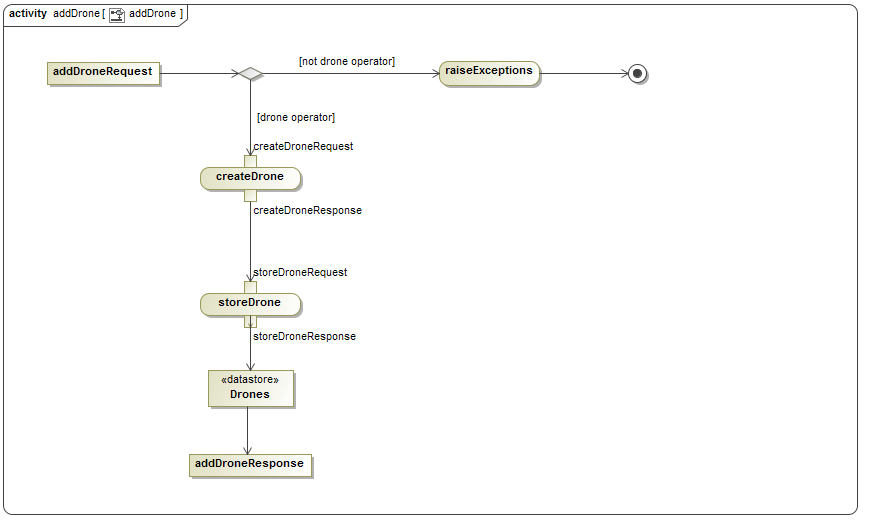
\includegraphics[width=\textwidth]{ps_add.png}  \\
			\caption{Process Specification : addDrone}
		\end{figure}
		\begin{figure}[H]
			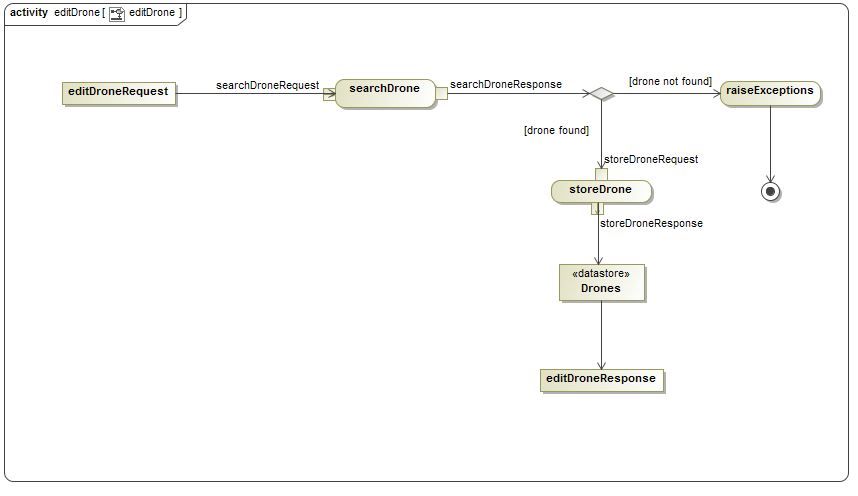
\includegraphics[width=\textwidth]{ps_edit.png}  \\
			\caption{Process Specification : editDrone}
		\end{figure}
		\begin{figure}[H]
			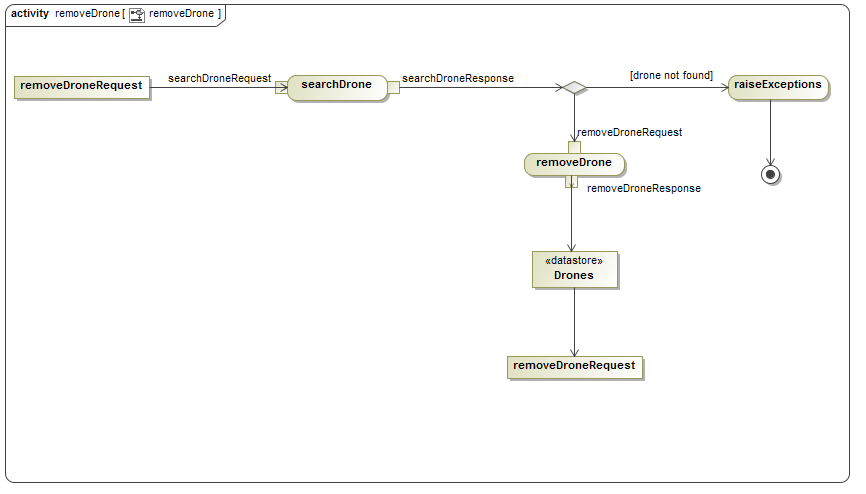
\includegraphics[width=\textwidth]{ps_delete.png}  \\
			\caption{Process Specification : removeDrone}
		\end{figure}
		%To include diagrams for process specifications here.
		
	
	
\newpage

	\subsection{Domain Model}
	
	The domain model shows the data structure requirements of the Researcher Support System, as well as the relationships between the different domain objects. 

	\begin{figure}[H]
		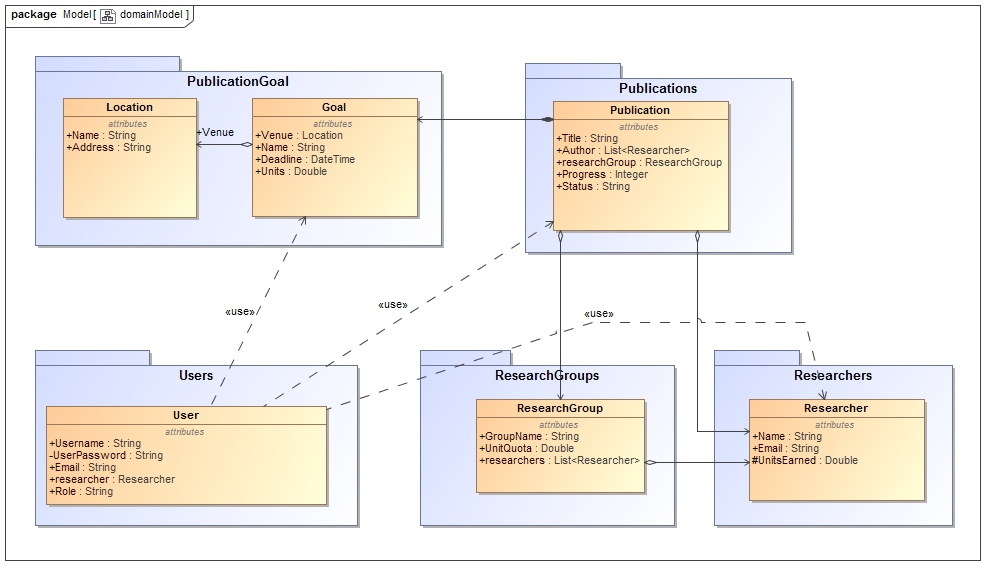
\includegraphics[width=\textwidth]{domainModelB.jpg}  \\
		\caption{Domain Model}
	\end{figure}
	
\newpage

\section{Mission subsection}
%\lable{sec:open}
\subsubsection{Use cases}

		\begin{flushleft}
			\textbf{Critical}
				\begin{itemize}
	  				\item Add mission
	  				\item Delete mission
	  				\item View mission
				\end{itemize}
				
				\begin{figure}[H]
					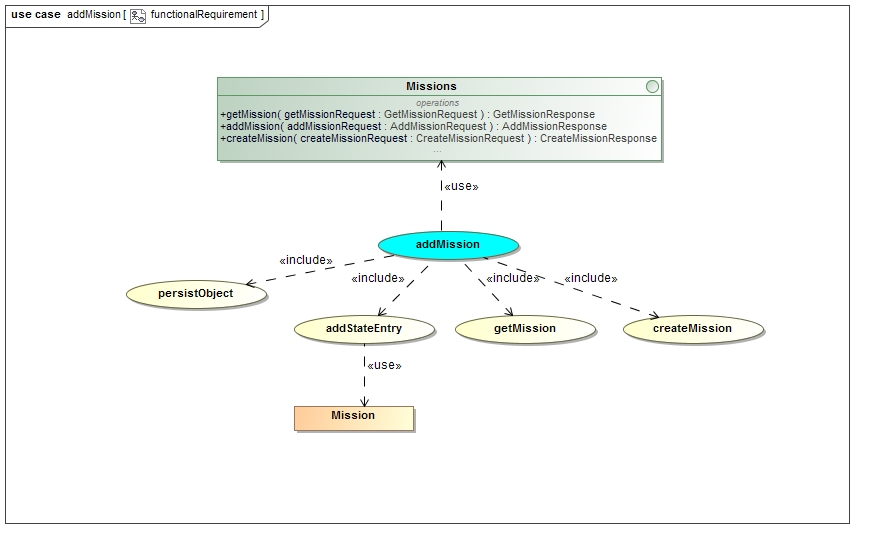
\includegraphics[width=\textwidth]{functionalRequirement_addmission.jpg}  \\
					\caption{Use case : addMission}
				\end{figure}
				
				\begin{figure}[H]
					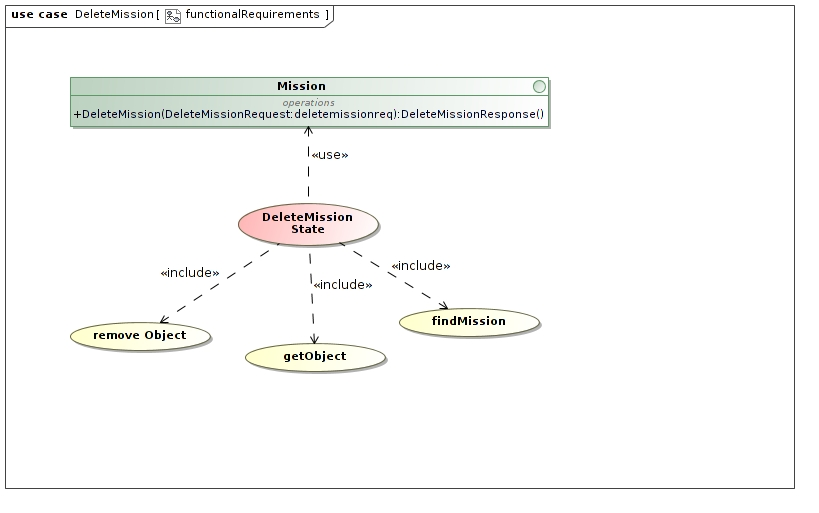
\includegraphics[width=\textwidth]{functionalRequirementsDeleteMission Use Case Diagram.jpg}  \\
					\caption{Use case : deleteMission}
				\end{figure}
				
				\begin{figure}[H]
					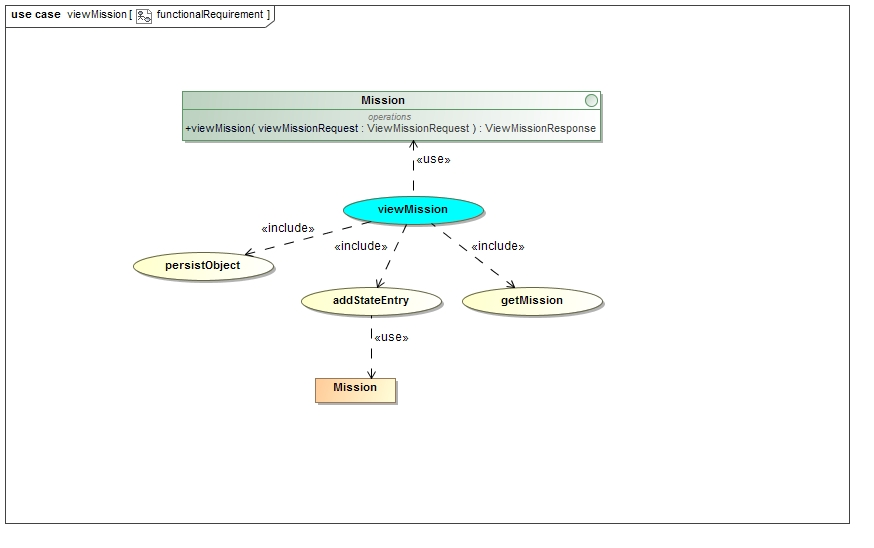
\includegraphics[width=\textwidth]{functionalRequirement_viewmission.jpg}  \\
					\caption{Use case : viewMission}
				\end{figure}

			\textbf{Nice-To-Have}
				\begin{itemize}
	  				\item Edit mission
				\end{itemize}
				
				\begin{figure}[H]
					\includegraphics[width=\textwidth]{functionalRequirementsEditmissin Use case Diagram.jpg}  \\
					\caption{Use case : viewMission}
				\end{figure}
		\end{flushleft}
\end{document}
